
\documentclass{bmcart}

\usepackage{amsthm,amsmath}
\usepackage[utf8]{inputenc}
\usepackage{url}
\usepackage{color}
\usepackage{xspace}

\def\includegraphic[#1]{}
\def\includegraphics[#1]{}


%%% Put your definitions there:
\startlocaldefs

\newcommand*{\eg}{e.g.\@\xspace}
\newcommand*{\ie}{i.e.\@\xspace}
\newcommand{\ipt}{IPT\xspace}
\newcommand{\ipts}{IPTs\xspace}

\newcommand{\patk}{p\mathrm{@}k}

\newcommand{\ml}[1]{\textcolor{blue}{ML: #1}}
\newcommand{\vl}[1]{\textcolor{red}{VL: #1}}
\newcommand{\ja}[1]{\textcolor{purple}{JA: #1}}

\endlocaldefs


%%% Begin ...
\begin{document}

%%% Start of article front matter
\begin{frontmatter}

\begin{fmbox}
\dochead{Research}

%%%%%%%%%%%%%%%%%%%%%%%%%%%%%%%%%%%%%%%%%%%%%%
%%                                          %%
%% Enter the title of your article here     %%
%%                                          %%
%%%%%%%%%%%%%%%%%%%%%%%%%%%%%%%%%%%%%%%%%%%%%%

\title{Learning Auditory Similarities Between Instrumental Playing Techniques}

%%%%%%%%%%%%%%%%%%%%%%%%%%%%%%%%%%%%%%%%%%%%%%
%%                                          %%
%% Enter the authors here                   %%
%%                                          %%
%% Specify information, if available,       %%
%% in the form:                             %%
%%   <key>={<id1>,<id2>}                    %%
%%   <key>=                                 %%
%% Comment or delete the keys which are     %%
%% not used. Repeat \author command as much %%
%% as required.                             %%
%%                                          %%
%%%%%%%%%%%%%%%%%%%%%%%%%%%%%%%%%%%%%%%%%%%%%%

\author[
   addressref={aff1},                   % id's of addresses, e.g. {aff1,aff2}
   corref={aff1},                       % id of corresponding address, if any
   noteref={n1},                        % id's of article notes, if any
   email={email@example.com}            % email address
]{\inits{CE}\fnm{Christian} \snm{El-Hajj}}
\author[
   addressref={aff2},
   email={email@example.com}
]{\inits{VL}\fnm{Vincent} \snm{Lostanlen}}
\author[
   addressref={aff2},
   email={email@example.com}
]{\inits{MR}\fnm{Mathias} \snm{Rossignol}}
\author[
   addressref={aff2},
   email={email@example.com}
]{\inits{GL}\fnm{Gr\'egoire} \snm{Lafay}}
\author[
   addressref={aff2},
   email={email@example.com}
]{\inits{ML}\fnm{Mathieu} \snm{Lagrange}}

%%%%%%%%%%%%%%%%%%%%%%%%%%%%%%%%%%%%%%%%%%%%%%
%%                                          %%
%% Enter the authors' addresses here        %%
%%                                          %%
%% Repeat \address commands as much as      %%
%% required.                                %%
%%                                          %%
%%%%%%%%%%%%%%%%%%%%%%%%%%%%%%%%%%%%%%%%%%%%%%

\address[id=aff1]{%                           % unique id
  \orgname{Department of Zoology, Cambridge}, % university, etc
  \street{Waterloo Road},                     %
  %\postcode{}                                % post or zip code
  \city{London},                              % city
  \cny{UK}                                    % country
}
\address[id=aff2]{%
  \orgname{Marine Ecology Department, Institute of Marine Sciences Kiel},
  \street{D\"{u}sternbrooker Weg 20},
  \postcode{24105}
  \city{Kiel},
  \cny{Germany}
}

%%%%%%%%%%%%%%%%%%%%%%%%%%%%%%%%%%%%%%%%%%%%%%
%%                                          %%
%% Enter short notes here                   %%
%%                                          %%
%% Short notes will be after addresses      %%
%% on first page.                           %%
%%                                          %%
%%%%%%%%%%%%%%%%%%%%%%%%%%%%%%%%%%%%%%%%%%%%%%

\begin{artnotes}
\note[id=n1]{Equal contributor}
\end{artnotes}

\end{fmbox}

%%%%%%%%%%%%%%%%%%%%%%%%%%%%%%%%%%%%%%%%%%%%%%
%%                                          %%
%% The Abstract begins here                 %%
%%                                          %%
%% Please refer to the Instructions for     %%
%% authors on http://www.biomedcentral.com  %%
%% and include the section headings         %%
%% accordingly for your article type.       %%
%%                                          %%
%%%%%%%%%%%%%%%%%%%%%%%%%%%%%%%%%%%%%%%%%%%%%%

\begin{abstractbox}

\begin{abstract}
Abstract here.
\end{abstract}

%%%%%%%%%%%%%%%%%%%%%%%%%%%%%%%%%%%%%%%%%%%%%%
%%                                          %%
%% The keywords begin here                  %%
%%                                          %%
%% Put each keyword in separate \kwd{}.     %%
%%                                          %%
%%%%%%%%%%%%%%%%%%%%%%%%%%%%%%%%%%%%%%%%%%%%%%

\begin{keyword}
\kwd{sample}
\kwd{article}
\kwd{author}
\end{keyword}

\end{abstractbox}

\end{frontmatter}

%%%%%%%%%%%%%%%%%%%%%%%%%%%%%%%%%%%%%%%%%%%%%%
%%                                          %%
%% The Main Body begins here                %%
%%                                          %%
%% Please refer to the instructions for     %%
%% authors on:                              %%
%% http://www.biomedcentral.com/info/authors%%
%% and include the section headings         %%
%% accordingly for your article type.       %%
%%                                          %%
%% See the Results and Discussion section   %%
%% for details on how to create sub-sections%%
%%                                          %%
%% use \cite{...} to cite references        %%
%%  \cite{koon} and                         %%
%%  \cite{oreg,khar,zvai,xjon,schn,pond}    %%
%%  \nocite{smith,marg,hunn,advi,koha,mouse}%%
%%                                          %%
%%%%%%%%%%%%%%%%%%%%%%%%%%%%%%%%%%%%%%%%%%%%%%

\section*{Introduction}
\label{sec:intro}

Music information retrieval operates at either of two levels: symbolic and auditory.
By resting on a notation system, the symbolic level facilitates the comparison of musical notes in terms of quantitative attributes, such as duration, pitch, or intensity at the source.
Timbre, in contrast, is a qualitative attribute of music, thus irreducible to a one-dimensional axis.
As a result, symbolic representations describe timbre indirectly, either via visuotactile metaphors (\eg{} dry, rough, bright, round, and so forth) or by specifying an instrumental playing technique (\eg{} bowed or plucked).

Despite their widespread use, linguistic references to musical timbre suffer from limited adequacy.
On the one hand, adjectives such as \emph{bright} or \emph{rough} are prone to misunderstanding, as they do not prescribe any musical gesture that is capable of achieving them.
On the other hand, the sole mention of playing technique does not determine any intended effect; and therefore, fails to generalize to the entire instrumentarium.
For instance, although the term \emph{breathy} alludes to a playing technique that is peculiar to wind instruments, a cellist may accomplish a seemingly breathy timbre by bowing near the fingerboard, i.e., \emph{sul tasto} in Italian.

The prospect of retrieving timbre perception across playing techniques necessarily exceeds the symbolic domain.
Instead, it involves a cognitive process which arises from the subjective experience of listening to music.
From the standpoint of audio signal processing, the task of simulating this cognitive process amounts to the design of a multidimensional feature space wherein some distance function evaluates arbitrary pairs of stimuli.
Rather than to merely discriminate instruments as mutually exclusive categories, this distance function must reflect a consensus of quantitative judgments of acoustic dissimilarity, all other parameters --- \ie{} duration, pitch, and intensity --- being equal.

Behind the overarching challenge of coming up with a robust predictive challenge for human behavior, the main practical application of timbre similarity retrieval lies in the emerging topic of computer-assisted instrumentation.
Following the aesthetic tradition of spectralism in contemporary music creation, the composer queries the machine with an arbitrary audio signal.
The outcome of this is an instrumental audio sample, alongside textual attributes of playing technique.
In this context, the computer serves as a bridge from the auditory level to the symbolic level, allowing to approximate a potentially infinite realm of timbral sensations by an orchestra of priorly specified extent and technical range.
To maximize the perceptual fidelity of such an approximation, a query-by-example search engine in the auditory domain should summarize the vastest possible vocabulary of timbral templates.

In this paper, we propose a machine listening model which computes the dissimilarity in timbre between any two audio samples.
The main originality of our model is that it encompasses a broad range of extended playing techniques, well beyond the so-called ``ordinary'' mode of acoustic production.
Specifically, we fit pairwise judgments for 78 different techniques arising from 16 instruments, some of which include removable timbre-altering devices such as mutes.
A second originality of our model is that we purposefully disregard the playing technique metadata underlying each audio sample during the training phase of our model.
Said otherwise, we rely on listeners, not performers, to define and evaluate the task at hand.

%% TODO: list Sections

%% TODO: mention companion website and open-source software



\section*{Timbre similarity judgments}
\label{sec:survey}

To construct a dataset for exploring the perception of timbre, we conducted a survey on the perceived similarity of a set of sounds.
The set consists of $78$ recordings of different instrument--PT (IPT) pairs, each played at the same pitch and nuance (for more information on the dataset, see the Dataset section).
\ja{Mathieu, which pitch and nuance?}%
In the survey, a subject asked to dots on a two-dimensional place in a free sorting task.
Each dot corresponded to a different IPT recording and was moved by the user dragging them with the mouse.
In addition to spatially arranging the dots, the user was also asked to assign one of $20$ colors to each dot, providing a simple clustering of the sounds.
While both the location and color of each dot was recorded, only the color was used in our subsequent analysis---the spatial arrangement was only used to facilitate the user's ability to organize the sounds.
More information on the data collection process is available in the Human timbre judgments section.

The above survey was implemented as an interactive website, links to which were sent out on internal mailing lists of the \emph{Conservatoire national sup\'erieur de musique et de danse de Paris} (CNSMDP) and international mailing lists focusing on research in audio and music processing.
We made the experiment available for two months, during which we obtained results for a total of $31$ subjects.
The final arrangement and color assignment of one of the subjects is shown in Figure \ref{fix:xp2display}.

\begin{figure}
\center
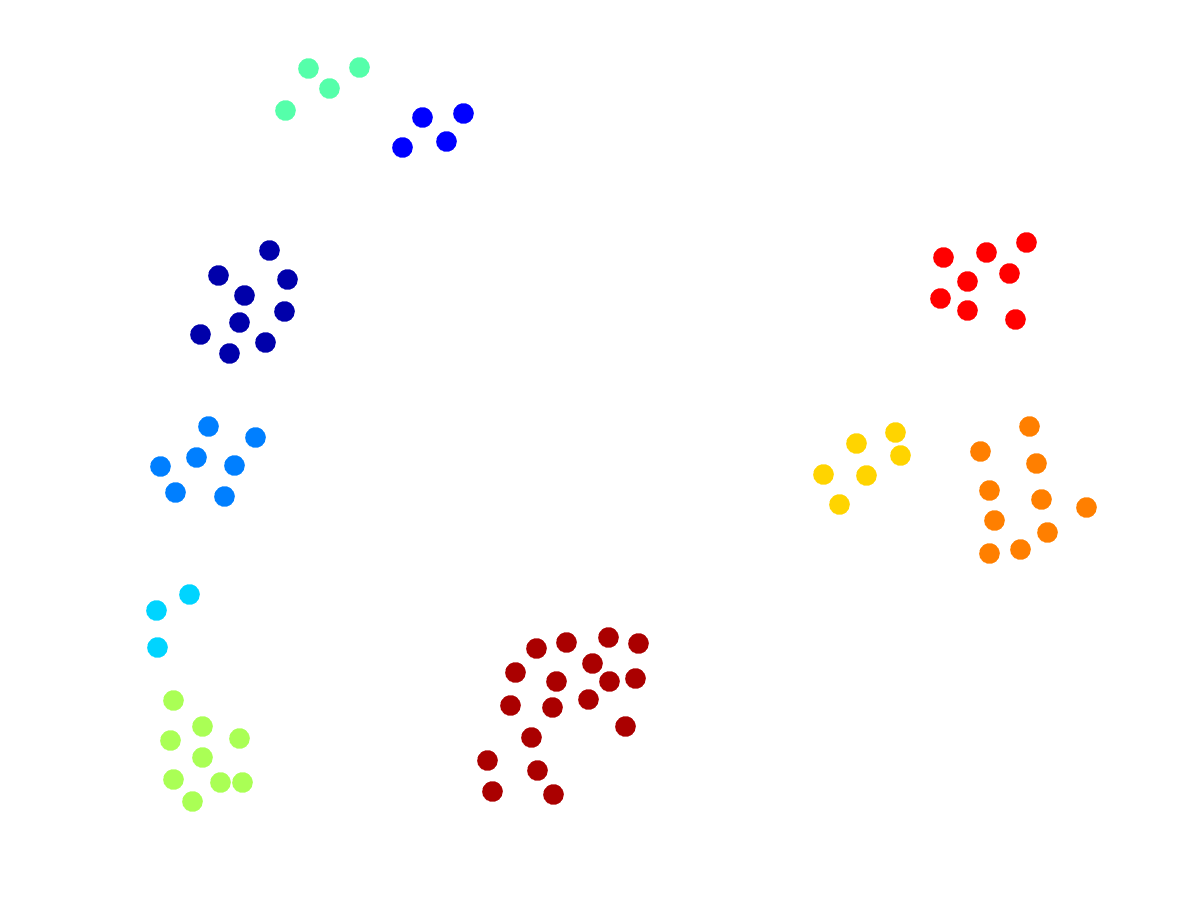
\includegraphics[width = \textwidth]{figures/xp2example1.png}
\caption{Spatial and group organization provided by subject 1.}
\label{fig:xp2display}
\end{figure}

For each subject, we constructed a matrix of size $78 \times 78$ to represent their similarity judgments for each pair of the $78$ IPTs.
Specifically, the $(i, j)$th element of the matrix was set to one if the $i$th and $j$th IPT were assigned the same color.
If not, it was set to zero.
In other words, we record the clustering assignment of each subject as a binary similarity matrix.

\ml{Joakim, equation needed ?}
\ja{I don't think so.
It should be fairly straightforward.}%

\ml{also have the resulting binary similarity matrix ?}
\ja{Yes, but I think we should have it for the consensus clustering described below.}%

Depending on the application, it may be of interest to condition the timbre space using the information of only one subject.
In this case, the correspondign binary similarity matrix may be used and the resulting timbre space is specialized to a given person.
It may also be of interest to condition the space using the aggregate similarity judgments given by several subjects.
That being said, conditioning the timbre space using several binary similarity matrices is not a trivial task, and will be discussed extensively in the Results section.
\ja{Why discuss it extensively there?
Don't we just settle on the partitioning algorithm below?}%

We found that using a hypergraph partitioning algorithm \cite{kernighan1970efficient,han1997scalable,strehl2002cluster} to produce the consensus similarity matrix performed well.
Interestingly, although several sounds pairs were obtained from the same instrument (but different PTs) and others were obtained using the same PT (but different instruments), the consensus clustering did not favor one of these taxonomies over the other.
\ja{We should have some figure to back this up.
Can this be done using the tag clouds?}

\section*{Proposed approach}
\label{sec:method}

\ml{introduce the system globally, while stressing the ability of the system to be conditionned for one or many people}

\subsection*{Scattering transform}
\label{sec:scattering}

While cortical representations have been successful in distinguishing properties of audio recordings (including similarity analysis and classification tasks), they remain models for the electrophysiological signals recorded in the audio cortex.
As such, their calculation is not always computationally efficient and their mathematical properties may be difficult to analyze directly.

A closely related representation is that of the time scattering transform, introduced by And\'{e}n and Mallat \cite{anden2011multiscale,anden2014deep}.
Given an audio recording, it decomposes the signal using an analytic wavelet transform and computes the modulus, obtaining the \emph{scalogram} of the signal.
The scalogram is similar to the spectrogram, but has a time--frequency resolution that varies with frequency: at low frequency, the filters are narrowly tuned in frequency (and hence wide in time), while at high frequency, the filters are wide in frequency (and hence narrowly concentrated in time).
This representation contains a large amount of information, but not in a form suitable for building statistical models.
In particular, the scalogram is not \emph{stable} in the sense that small deformations to the original signal may induce large changes to the scalogram.
It also lacks \emph{invariance} to time-shifting, which does not affect our perception of a sound, and should therefore not affect its timbre model.
One way to resolve this is to average the scalogram in time to obtain a spectral profile of the signal, yielding the first-order scattering coefficients.
These possess both invariance to time-shifting and stability to time-warping deformations \cite{anden2014deep}.

Since these first-order coefficients only include spectral information, they cannot accurately characterize more sophisticated structure in the signal.
One way to augment them is to calculate another wavelet decomposition in time, this time on each frequency channel of the scalogram.
Again, we compute the modulus of the wavelet coefficients and average in time.
The resulting coefficients are known as the second-order time scattering coefficients.
These also possess the desired invariance and stability properties, but capture more information on the temporal structure of the scalogram \cite{anden2014deep}.

While richer than a simple spectral decomposition, such as MFCCs, the second-order time scattering coefficients described above primarily capture structure in time.
Indeed, they do not explicitly encode frequency structure in an invariant and stable manner.
If a signal is transposed or warped in frequency by a small amount, we do not expect its timbre to change significantly.
We would therefore like our representation to have the same invariance and stability properties along the frequency axis.
This is achieved by taking first- and second-order scattering coefficients and computing a second scattering transform, this time along the log-frequency axis.
The resulting coefficients are known as separable time and frequency scattering coefficients \cite{anden2014deep}.

This representation does possess the desired invariance and stability properties, but its separable nature limits its power to adequately represent time--frequency structures that do not separate cleanly in time and frequency, such as chirps.
To remedy this, another approach was suggested by And\'{e}n et al. \cite{anden2015joint,anden2019joint} wherein the temporal wavelet decomposition of the scalogram is replaced with a two-dimensional, spectro-temporal decomposition.
Similarly to the cortical representation, the result is a four-dimensional array indexed by time, acoustic frequency, modulation frequency (or \emph{rate}), and spectral modulation frequency, known as \emph{quefrency} (or \emph{scale}).
As before, we compute the modulus and average in time, obtaining a set of coefficients known as second-order joint time--frequency scattering coefficients.

The definition of the scattering transform in terms of wavelet decompositions and modulus nonlinearities presents several advantages.
On the computational side, the critical bandwidth guarantees of wavelet transforms allows us to judiciously subsample the output, resulting in a lower-dimensional representation compared to the cortical representations.
The scattering transform also satisfies the aforementioned stability conditions, providing a guarantee that slightly deforming a signal only results in a negligible change in its scattering transform.
Furthermore, we may calculate the scattering tranforms of several model signals, including amplitude-modulated harmonic sounds and noise excitations \cite{anden2012scattering,anden2014deep}, frequency-modulated sinusoids (e.g., chirps) \cite{anden2012scattering,anden2019joint}, and beating phenomena \cite{anden2014deep}.
They have also enjoyed success in several audio classification and similarity retrieval tasks \cite{anden2011multiscale,bauge2013representing,anden2014deep,anden2019joint,lostanlen2018relevance,lostanlen2018extended}.

To evaluate the ability of the scattering transform to characterize the timbre of an audio signal, we consider the task of classifying musical notes from a wide variety of instruments played according to a set of extended instrumental playing techniques (IPTs).
Increasing the variability in IPTs allows us to explore a wider range of timbre, providing a more robust validation of the proposed model for modeling timbre.
The metric used is the \emph{precision at rank $k$} ($\patk$), which is calculated by computing the $k$ nearest neighbors in the feature space and recording the proportion of the neighbors that are in the same class.
In the following, we set $k = 5$.
The classes were obtained from the consensus clustering of human similarity judgments described in the previous section.
The $\patk$ therefore provides a measure of consistency between the timbre similarity measures obtained by our model and those of the survey subjects.

Concatenating the first- and second-order separable time and frequency scattering coefficients, we obtain a feature vector of dimension $???$ for a sound recording of duration $???$.
Computing nearest neighbors with the standard Euclidean measure gives a $\patk$ of $0.870 \pm 0.058$, where the first value indicates the mean and the second the standard deviation.
As a result, this simple transformation of the original signal results in a representation that lends itself naturally to discriminating timbre.
Note that this result is obtained by simply looking at the raw feature vectors---no learning is performed to adapt the transform towards discriminating timbre.
Replacing the separable second-order coefficients with the joint second-order coefficients boosts the $\patk$ to $???$.
This is evidence that accurately characterizing the joint time--frequency structure of the sound is important capturing its timbre.

We performed the same evaluation with a standard MFCC representation, obtaining a $\patk$ of $0.851 \pm 0.062$.
As a result, we conclude that a Euclidean distance over scattering transforms (separable or joint) yield little additional perceptual information compared to standard spectral descriptors.

\subsection*{Similarity weighting}
\label{sec:weighting}

To improve our measure, we need to replace the standard Euclidean distance on the raw scattering coefficients by something better adapted to discriminating timbre.
Equivalently, we can apply further transformations to the scattering coefficients and compute the Euclidean distance on the result.
Very flexible and powerful methods can be brought to bear on this problem, such as deep neural networks, but with their flexibility comes an increase in complexity.
This increased complexity of the model reduces its usefulness with respect to interpretability.

For this reason, we restrict ourselves to a simple linear transform of the scattering coefficients.
Specifically, we construct a positive semidefinite matrix $L$ that we apply to the scattering coefficients $x$ so that the Euclidean distance between $Lx$ and $Ly$ best approximates the consensus clustering obtained above.
We expect the resulting representation $Lx$ to provide a more accurate model for timbre perception.

We now use the consensus clustering to reweight the similarity between feature vectors (either MFCCs or scattering transforms).
For this, we use the \emph{large margin nearest neighbor} (LMNN) metric learning algorithm \cite{weinberger2006distance, weinberger2009distance}.
This approach constructs a positive semi-definite weighting matrix $L$ such that the distance $\|Lx - Ly\|$ best classifies a set of points into a fixed clustering assignment.
Running LMNN on MFCCs with the consensus clustering obtained above increases $\patk$ slightly to $0.862 \pm 0.059$.
Consequently, there seems to be little additional timbre information in the MFCCs compared to that given by the standard Euclidean distance.
We contrast this with LMNN applied to the separable scattering coefficients, which yields a $\patk$ of $0.948 \pm 0.033$, which is a significant increase.
For the joint scattering coefficients, we obtain a $\patk$ of $???$.
We therefore conclude that a simple reweighting of the scattering transform yields a more appropriate timbral similarity measure.

\section*{Results}
\label{sec:results}

\ja{The results are currently sprinkled into the above methods section.
These need to be extracted and summarized here.}

post processing

std consisten across features
mfcc cut
consistent with [previous papers] each item provides incremental gain of perforamnces

table 3 valeurs erreur

ablation study

tfscat+lmnn
tfscat
scat

9 pas de weighting averaging not end to end

separate pas trop de perte : consensus bon

perf du best tool chain on complete dataset

randomize

perf on 50/50

lda

-lmnn

tf -> scat

tfscat -> mfcc + etendus



\section*{Discussion}
\label{sec:discussion}

\begin{itemize}
\item Demonstrates complex timbral structure perceived by subjects in study: neither instrument (i.e., spectral envelope) or playing technique (i.e., temporal modulation) dominates similarity judgment. Need joint to characterize time-frequency structure (see Patil et al).
\item Proposed computational model (scattering + linear) reproduces similarity judgments accurately. Easy to ``retrain'' for other data. Fixed wavelet structure allows for analysis of linear layer and guarantees invariance and stability properties.
\item Applications: query-by-example in musical sample databases.
\end{itemize}

%%%%%%%%%%%%%%%%%%%%%%%%%%%%%%%%%%%%%%%%%%%%%%
%%                                          %%
%% Backmatter begins here                   %%
%%                                          %%
%%%%%%%%%%%%%%%%%%%%%%%%%%%%%%%%%%%%%%%%%%%%%%

\begin{backmatter}

\section*{Competing interests}
  The authors declare that they have no competing interests.

\section*{Author's contributions}
    Text for this section \ldots

\section*{Acknowledgements}
The Flatiron Institute is a division of the Simons Foundation.

%%%%%%%%%%%%%%%%%%%%%%%%%%%%%%%%%%%%%%%%%%%%%%%%%%%%%%%%%%%%%
%%                  The Bibliography                       %%
%%                                                         %%
%%  Bmc_mathpys.bst  will be used to                       %%
%%  create a .BBL file for submission.                     %%
%%  After submission of the .TEX file,                     %%
%%  you will be prompted to submit your .BBL file.         %%
%%                                                         %%
%%                                                         %%
%%  Note that the displayed Bibliography will not          %%
%%  necessarily be rendered by Latex exactly as specified  %%
%%  in the online Instructions for Authors.                %%
%%                                                         %%
%%%%%%%%%%%%%%%%%%%%%%%%%%%%%%%%%%%%%%%%%%%%%%%%%%%%%%%%%%%%%

\bibliographystyle{bmc-mathphys}
\bibliography{bib}

%% Appendices

\section*{Dataset}
\label{sec:dataset}

The dataset considered in this paper as been recorded at Ircam and is composed of audio recording of $16$ different musical instruments played with different PTs, which leads to $235$ different IPT pairs.
In addition, the pitch and nuance is varie for each pair (when applicable), yielding a total of $25444$ audio recordings.
For each couple, the pitch and intonation is varied leading to 25444 audio samples.

The recorded instruments belongs to the wind and string classes.
For winds, the instruments considered in the second experiment are: accordion (Acc), saxophone alto (ASax), tuba (Tb), bassoon (Bn), clarinet Bb (BbCl), flute (Fl), horn (Hn), oboe (Ob), trombone tenor (TTbn), and trumpet C (TpC).
For the string class, the instruments are: guitar (Gtr), harp (Hp), viola (Va), violin (Vn), violoncello (Vc), and contrabass (Cb).
\ja{Better to display these in a table?}

Some instruments can be complemented with sordina (S), wha (W).
The addition of this kind of device modifies the shape of the instrument.
Consequently, an alto saxophone and alto saxophone with sordina are considered as different instruments.
\vl{This is crucial and should not be deferred to the appendix. @writing}
\ml{J'ai mis ca en appendice pour ne pas que le lecteur confonde la base SOL complete et les données considérées dans l'étude.}

Those instruments are recorded for different nuance and pitch if the latter is relevant, but more importantly, several playing technique are considered.
For the second experiment described in this paper, the playing techniques considered are: artificial harmonic (art), blow (blow), exploding slap (explo), harmonic (harm), key-click (key), col legno (legno), non vibrato (nonvib), ordinario (ord), pedal tone (pdl), pizzicato (pizz), ponticello (pont), slap (slap), (tasto), tongue-ram (tng), and xylophonic (xyl).

\vl{This section is not precise enough in terms of intensity ranges and pitch ranges.
The abbreviations can be removed. @data @writing}
\ml{}

\vl{A bubble plot of number of notes per instrument (x axis) and playing technique
(y axis) would be extremely useful. @data @figure}
\ml{Tu voudrais ca pour la base SOL complete ou les données considérées dans l'étude ?}
\vl{Les donn\'{e} de l'\'{e}tude, relatives aux Figures 5 et 6.}

\section*{Human timbre judgments}
\label{sec:subjective}

The dataset considered in this study is taken
from the studio-on-line (SOL) music library  \cite{peeters2000instrument}.
It has audio recordings of 16 different musical instruments played
with different playing techniques,
which leads to $235$ different couples of instrument / playing technique.
For each couple, the pitch and intonation is varied leading to $25444$ recordings.
The way the dataset is structured
is explained in more details in Appendix \ref{sec:dataset}.

Gathering the similarity judgments between each pair of samples would be a daunting task. Indeed, studies about perceptual similarity are hindered with a dimensional problem as the number of pairs to be evaluated grows with the square of the number of items considered.

One reasonable assumption that we choose to consider here is that the pitch and nuance do not alter significantly the perception of timbral similarity. This is in line with the ANSI negative definition of timbre \vl{expliquer, citer, et modérer le propos en donnant des exemples dans lequel le pitch ou la nuance change le timbre}.


\section*{Reducing Expert judgments of technique peculiarities}

\ja{This needs to be summarized (possible in the previous section).
I'm copying two sentences in here that I had in the Timbre similarity judgments section.}%
These IPTs were selected from a larger set of $235$ IPTs by two experts at the \emph{Conservatoire national sup\'erieur de musique et de danse de Paris} (CNSMDP).
The selection criteria were based on the likelihood of an IPT being similar to some other IPT, ensuring that IPTs that were too singular were excluded from the survey.

Even so, considering every pairs of IPTs is not practical. A selection
experiment is thus conducted where the subject is asked to give his opinion on which
\ipts are relevant to study. More precisely, an \ipt is said to be relevant to study
if it is likely to be associated to another \ipt of another instrument.
Interest is rated on a 7 ticks scale. The subject can listen to all the different
nuance and pitch samples of each \ipt. The experiment is over when all the
\ipts are rated.

Rating guidelines are provided :
\begin{itemize}
  \item One star: this \ipt is singular, it is not useful to compare it with another \ipt of another instrument.
  \item Four stars: there is a proximity on one aspect of the sound between this
  \ipt and of an \ipt of another instrument,
  but this one is neither decisive nor obvious.
  \item Seven stars: there is a large similarity between this \ipt and an \ipt of another instrument.
\end{itemize}

Two music composition professors of the CNSMDP performed the test, that is rating each $235$ \ipt.

\vl{This subsection needs a box-and-whisker plot of ratings, where the 235 different
couples of instrument and playing techniques are sorted on the x-axis by average rating. @figure @ratings}

\ml{il n'y que deux raters, ca ne pas pas sens de faire et ca sera illisible}

\vl{Are the histogram of ratings similar for the two raters? It would be good to make a statistical test for this. @research @stats @ratings}

\ml{les histograms sont dans la figure statxp1. Le code pour la generer est dans code/xp1 faire tourner extractData et statData. Un ttest rejette l'hypothese nulle.}

Even if the hypothesis that the distributions of ratings comes from independent random samples from normal distributions with equal means and equal but unknown variances, is verified using the two-sample t-test, inspection of the respective histograms reveals that averaging the ratings of the two raters is reasonable.

Keeping in mind that the gathering of the perceptual judgments of \ipt similarities shall remain practical, the number of \ipts considered shall be lower than $100$. We thus select the \ipts with an average rating higher than three, which brings us 78 \ipts to study.

%%%%%%%%%%%%%% CROWDSOURCED JUDGMENTS OF PAIRWISE SIMILARITY %%%%%%%%%%%%%%%%%%%%
\section*{Crowdsourced judgments of pairwise similarity}

\ja{A lot of this is covered in the main text.
Not sure what we need to add in the appendix.}

The second experiment aims at gathering spontaneous judgment of similarity for those 78 \ipts using a canonical free sorting task. This type of task is chosen among others for two main reasons. First, it gives the ability to the subject to listen to the whole set of \ipts before performing the task. Second, it gives more freedom to the subject, thus potentially more interest to perform the task than a lengthy series of XXY dissimilarity ratings.

The subjects are thus asked to organize the 78 \ipts displayed as grey dots on a two dimensional plane into groups by assigning colors to each dots according to their "acoustic similarity". The textual instructions provided to introduce the experiment was chosen to be deliberately vague in order to allow the subject to follow its own judgment.

The plane is displayed on a computer screen using a web based interface\footnote{The interface is available here: http://soundthings.org/ticel/groupSounds}. The \ipts can be listened to by hovering the mouse on the corresponding dot. The experiment is over when the subject assigned a color to all the dots. The initial location of the dots on the plane is randomized for each subject and can be changed during the experiment by the subject for convenience. Event hough the location of the dots is recorded, this data is not considered during the analysis.

The experiment was available online for two months and requests to perform the test have been sent to internal mailing lists of the CNSMDP and international research mailing with a focus on audio and music processing. The experiment have been performed on a voluntary basis without gratification. Subjects were asked to use headphones at a comfortable listening level.


31 subjects completed the experiment. An example of resulting organization of \ipt is given on Figure \ref{fig:xp2display}. \footnote{The resulting organization for each subject are available for reader's inspection using the full feature interface provided to the subjects for performing the experiment \url{https://mathieulagrange.github.io/paperSpontaneousSimilarity/demo}}.

As only the clustering given by the subjects using the color labels is considered to estimate the spontaneous judgments of similarity among \ipt. The spatial organization of the dots representing the \ipt could provide information about the similarity, but this would implicitly enforce the fact that the timbral similarity space is two dimensional. We therefore now only study the properties of the clusterings performed by the subject prior to converting them into an overall similarity matrix.

This results in $31$ clusterings that can be considered for defining a perceptual timbre space of \ipts.


\section*{Analysis}\label{sec:analysis}

\ja{I thought all of this stuff was going away and we were just replacing it with a brief analysis using the tag clouds (and so on).
At any rate, the relevant analysis results should be in the main text (under Timbre similarity judgments, after we describe the experiments).}%

In order to gain information about the relevance those $31$ clusterings for defining a perceptual timbre space of \ipts, an analysis is performed.

Among the 20 colors available, the subjects used on average $10.2 \pm  4.1$ different colors to group \ipts. The distribution of the number of groups can be seen on Figure \ref{fig:xp2nbGroup}. The size of the groups is on average $7.7 \pm   7.2$. The distribution of the size of groups can be seen on Figure \ref{fig:xp2sizeGroup}. The large number of small groups indicates that many subjects considered that a few of the \ipt were very different from all the remaining \ipt.

\begin{figure}
\center
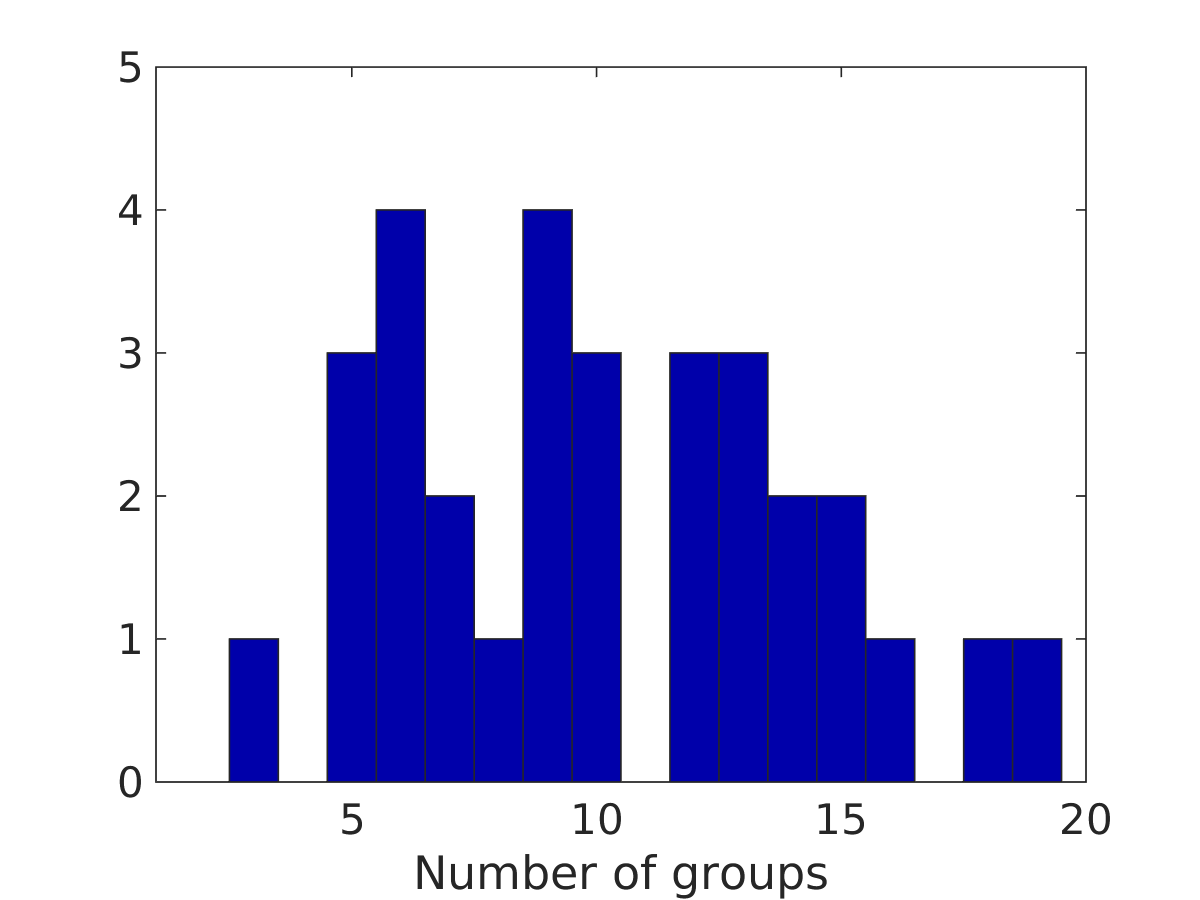
\includegraphics[width = \textwidth]{figures/nbc.png}
\caption{Histogram of the number of groups.
\vl{The width of this figure should be a half page instead of a full page. Pair with next figure. @figure}}
\ml{ok}
\label{fig:xp2nbGroup}
\end{figure}

\begin{figure}
\center
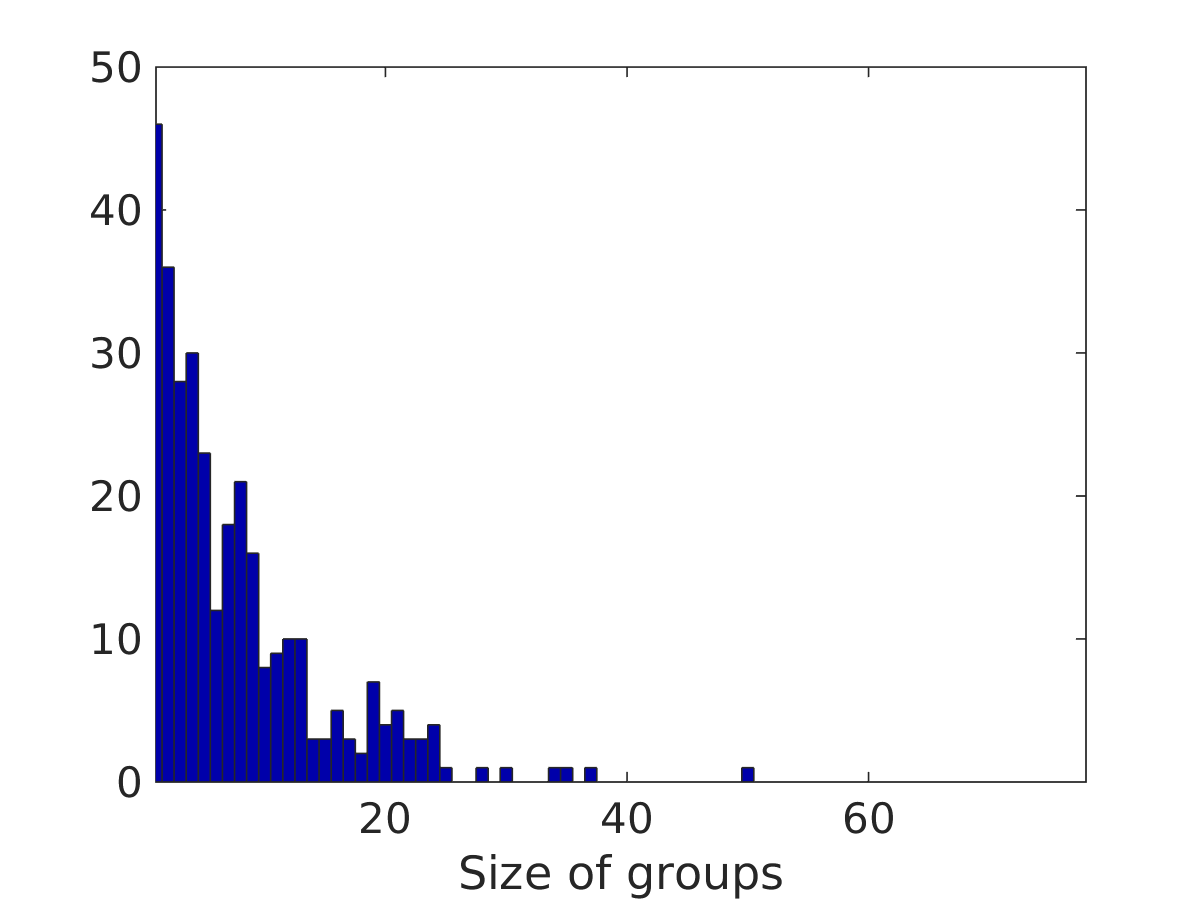
\includegraphics[width = \textwidth]{figures/sbc.png}
\caption{Histogram of the size of groups.
\vl{The width of this figure should be a half page instead of a full page. Pair with previous figure. @figure}}
\ml{ok}
\label{fig:xp2sizeGroup}
\end{figure}

A clustering can be considered as a binary similarity measure, with $s(a, b) = 1$ if $a$ and $b$ belong to the same group, and $0$ otherwise. By averaging the 31 binary similarity matrix, an overall floating point matrix is obtained that corresponds to our measure of the spontaneous perceptual similarity between \ipt.

In order to gather information about the properties of the data, a cluster analysis is next performed using an agglomerative hierarchical clustering \cite{gordon1987review} using the weighted average algorithm for computing distance between clusters. The resulting dendrogram is displayed on Figure \ref{fig:dendrogram}. A partition of $n$ clusters can be constructed from the agglomerative hierarchical cluster tree by finding the smallest height at which a horizontal cut through the tree leaves $n$ clusters.

One question that arises is whether the similarity is influenced primarily by the instrument or by the playing technique. To answer this question, each partition provided by cutting the dendrogram at successive levels is compared to two reference partitions. One reference is the partition of the \ipts when labeled with the instrument used (I) and the other if the partition of the \ipts when labeled with the playing technique used (Pt).

There are many metrics available to compare two partitions by evaluating their degree of correspondence \cite{wagner2007comparing}. The normalized mutual information (NMI) is interesting as it do not require alignement of the groups labels between the two partitions prior correspondence analysis and the two partition are not required to have the same number of groups. It also by design bounded between 0 and 1, 1 meaning perfect match. We consider the normalization proposed in \cite{strehl2002cluster}. Figure \ref{fig:clusters} shows the evolution of the NMI when comparing the partitions provided by the cluster analysis of the dendrogram produced using the human judgment of similarity and respectively the instrument partition ($j/I$) or the playing technique partition ($j/Pt$).

\begin{figure}
\center
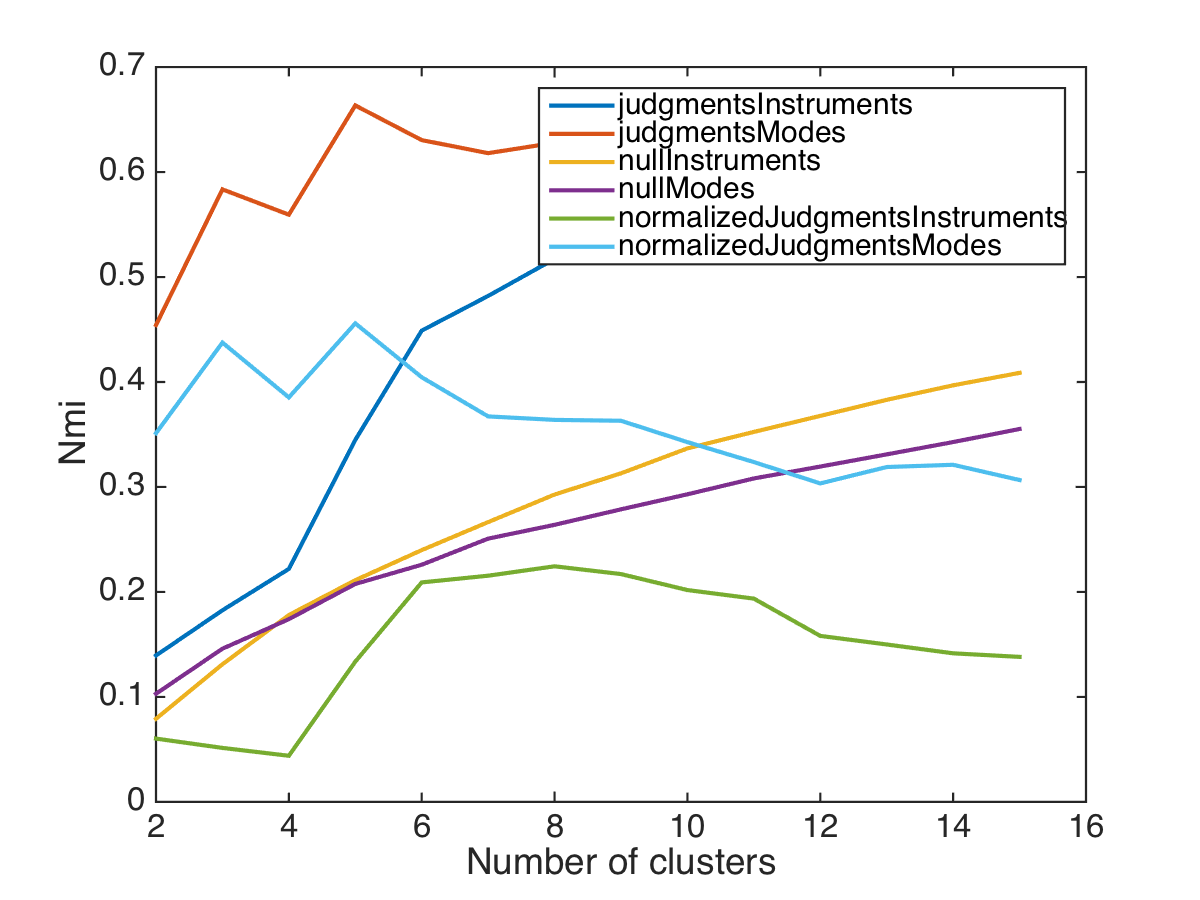
\includegraphics[width = \textwidth]{figures/clusterAnalysis.png}
\caption{Cluster analysis of the similarity judgments. $j/I$ and $j/Pt$ compare the partition obtained using the similarity judgments clustered using a growing number of clusters versus respectively the instrument partition and the playing technique partition. Normalizing null partitions based NMI $nullI$ and $nullPt$ are used to obtain normalized measures: $nj/I$ and $nj/Pt$.
\vl{This line plot is very hard to understand.
The legend box occludes the data on the top-right corner.
It would be preferable to remove this legend box and label lines
by placing text upon them,
so that the plot would be legible to readers with color vision deficiencies.
Besides, the choice of line labels is cryptic, as it relies on abbreviations.
The distinction between I and Pt
can be illustrated by two complementary colors, \eg{} blue versus orange.
The distinction between j, nj, and null
can be illustrated by three distinct markers
(empty circle, filled triangle, asterisk),
associated with
three distinct line styles (solid, dashed, dotted).
The NMI abbreviation should be expanded.
@figure}}
\ml{ok, le .fig est dispo}
\label{fig:clusters}
\end{figure}

There is a clear gain of NMI when considering the playing technique which means that the subjects primarily used cues corresponding to the playing technique to organize the \ipts. Also, for both curves, a global trend of increase in the $j/x$ partitions with respect to the number of clusters can be observed. This is a well documented fact, which simply put, means that it is easier to match any given partition with more clusters at hand \cite{tibshirani2001estimating}. To compensate for this bias, one can consider the NMI that would be achieved by comparing to the reference partition several random partitions of increasing number of clusters. The resulting averaged NMI for 100 randomly generated partitions is displayed on Figure \ref{fig:clusters}. This so-called null partitions NMI are respectively termed $nullI$ and $nullPt$ depending on the reference used. To normalize $j/I$ and $j/Pt$ in order to reduce the impact of this bias, we simply subtract the $null$ NMI:
\begin{eqnarray}
  nj/I &=& j/I - null \\
  nj/Pt &=& j/Pt - null  \\
\end{eqnarray}
This normalization is useful for identifying more easily the number of clusters for which the comparison is most relevant. As can be seen on Figure \ref{fig:clusters}, the number of clusters that leads to the highest NMI is 5 for the playing technique reference and 8 for the instrument reference, leading respectively to an NMI of $0.46$ and $0.21$. For the latter, reducing the number of clusters down to 6 do not decrease the NMI by much, a fact that will be latter discussed in more details. Even by considering the null normalization, the matching level is much higher for the playing technique reference.

The correspondences between those partitions and the reference ones are now studied. For this purpose, Figure \ref{fig:gi} displays two partitions. At the bottom is the partition that corresponds to the instruments labels, whose color code is given by the color bar on the right. The abbreviations used for the instruments are detailed in Section \ref{sec:dataset}. The ordering of \ipts on the horizontal axis is the one given by the cluster analysis, see the dendrogram on Figure \ref{fig:dendrogram}. The partition on top is the result of the clustering with 8 clusters. For visualization purposes, we arbitrarily set colors to clusters of this partition to the color code of the instrument label that is most often encountered in this cluster. If some labels occur equally often, the instrument of the first \ipt of the cluster is chosen. The emerging instrument classes are: Saxophone, Clarinet, Trumpet, Flute and Cello.

However, even with an optimal number of clusters, we see that the clusters have  a low purity, \ie{} a very diverse set of instruments labels for the \ipt they belong to. Also, some clusters could be merged without strong changes in the overall organization. This probably explains the small changes of NMI when reducing the number of clusters, see Figure \ref{fig:clusters}.

As can be seen on Figure \ref{fig:gm}, the correspondence between the playing technique reference and the resulting partition with 5 clusters is much higher. Most clusters have a high level of purity and for groups emerge : Pizzicato, Slap, Ordinario, and Ponticello.

To conclude this section, the process of gathering data about the perceptual similarity of \ipt is found to be successful as the subjects used their degree of freedom in a consistent manner and no inconsistency in the data has been detected during the analysis process. The main result is that the playing technique is an important factor when modeling the spontaneous judgment of similarity gathered in the second experiment.


\begin{figure}
\center
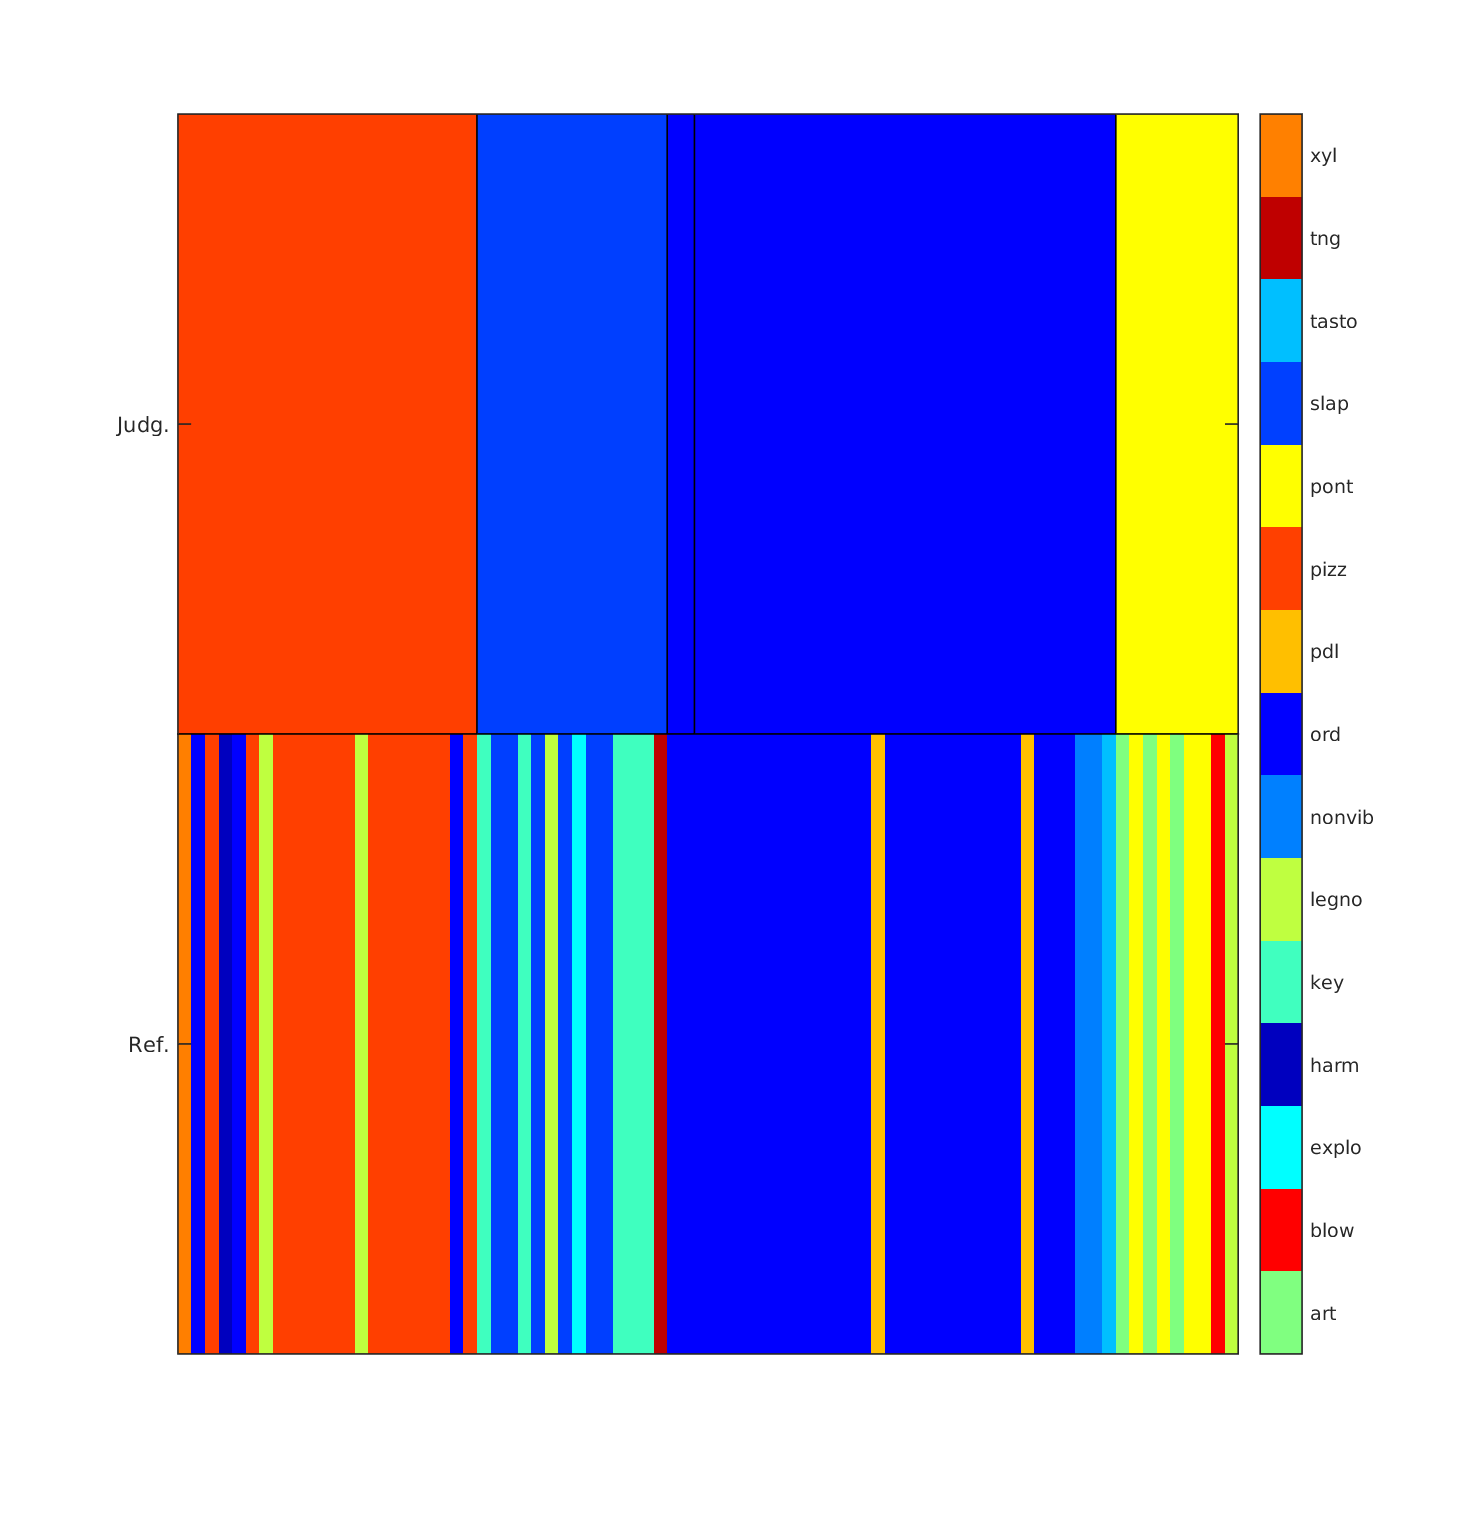
\includegraphics[width = \textwidth]{figures/groupModes.png}
\caption{Clustering \ipts using average perceptual similarity into 5 clusters (top) and playing technique labels (top). The color chosen to display each clusters on top corresponds to the playing technique that is dominant in this cluster, from left to right: 'pizzicato', 'slap', 'key', 'ordinario', 'ordinario', 'ponticello', 'art'.
\vl{A bubble plot would be preferable to a color map. Abbreviated words should appear in their expanded form instead. @writing}}
\ml{Je demande a voir, mais je ne suis pas satisfait de cette visu de toute facon. Le code est dispo dans le rep code. Lancer ticelSim en premier.}
\label{fig:gm}
\end{figure}





\begin{figure}
\center
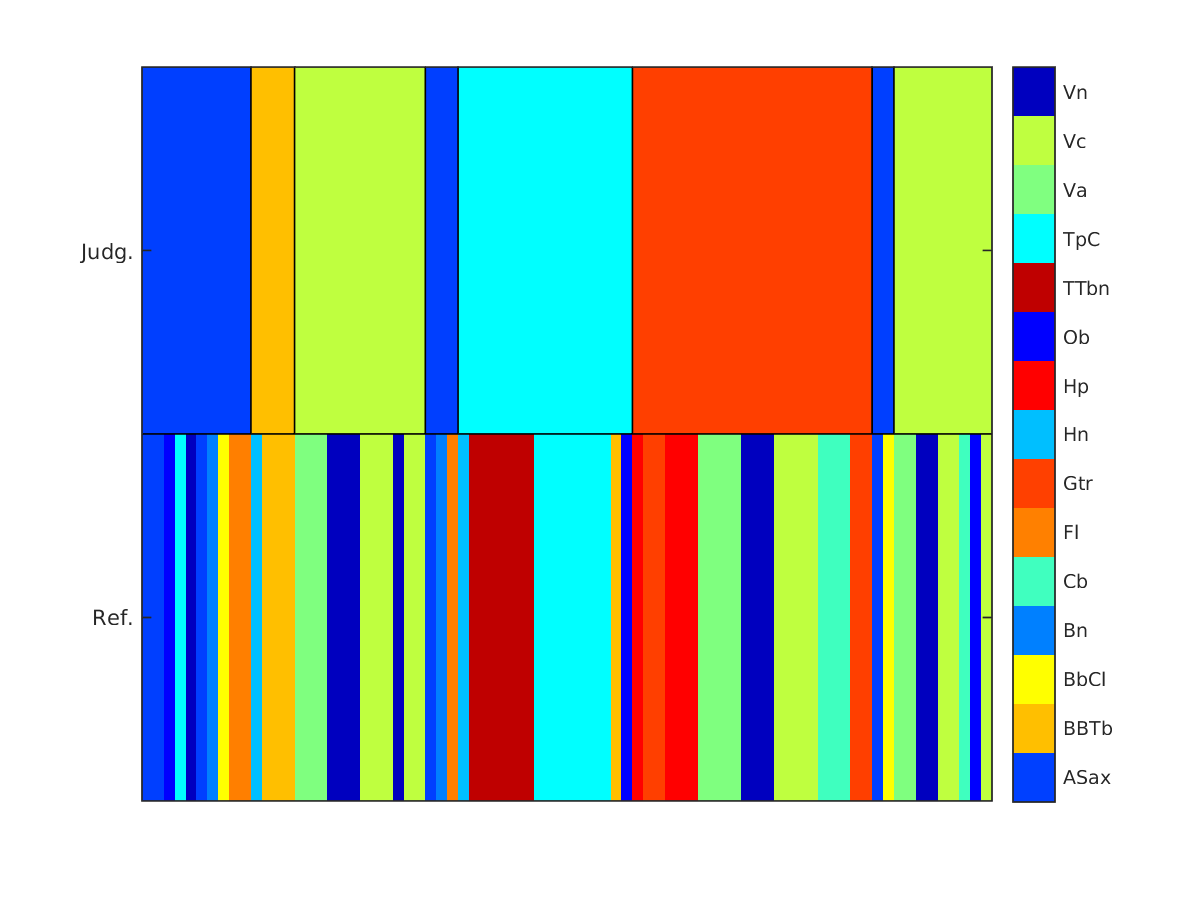
\includegraphics[width = \textwidth]{figures/groupInstruments.png}
\caption{Clustering \ipts using average perceptual similarity into 8 clusters (a) and instrument reference labels (b). The color chosen to display the groups (on top) corresponds  to the instrument that is dominant in this group, from left to right: 'ASax', 'BBTb', 'Vc', 'ASax', 'TpC', 'Gtr', 'ASax', 'Vc'.
\vl{A bubble plot would be preferable to a color map. Abbreviated words should appear in their expanded form instead. @writing}}
\ml{ok}
\label{fig:gi}
\end{figure}



%%%%%%%%%%%%%%%%%%%%%%%%%%%%%%%%%%%
%%                               %%
%% Figures                       %%
%%                               %%
%% NB: this is for captions and  %%
%% Titles. All graphics must be  %%
%% submitted separately and NOT  %%
%% included in the Tex document  %%
%%                               %%
%%%%%%%%%%%%%%%%%%%%%%%%%%%%%%%%%%%

\section*{Figures}

\begin{figure}[h!]
\caption{\csentence{STRF + scattering (upsampling STRF)}
A short description of the figure content should go here.}
\end{figure}

\begin{figure}[h!]
\caption{\csentence{Model overview}
One line music players (3 ipts bass pizz, bass archo, violin archo) sound, spec,
scat, isomap.
Second line : perceptual clustering.}
\end{figure}

\begin{figure}[h!]
\caption{\csentence{Sample scattering}
Same 3 sounds spec + scatt.}
\end{figure}

\begin{figure}[h!]
\caption{\csentence{Tag clouds}
A short description of the figure content should go here.}
\end{figure}

\begin{figure}[h!]
\caption{\csentence{Perfs MFCC, separable, joint (last)}
A short description of the figure content should go here.}
\end{figure}

%%%%%%%%%%%%%%%%%%%%%%%%%%%%%%%%%%%
%%                               %%
%% Tables                        %%
%%                               %%
%%%%%%%%%%%%%%%%%%%%%%%%%%%%%%%%%%%

\section*{Tables}
\begin{table}[h!]
\caption{Sample table title. This is where the description of the table should go.}
      \begin{tabular}{cccc}
        \hline
           & B1  &B2   & B3\\ \hline
        A1 & 0.1 & 0.2 & 0.3\\
        A2 & ... & ..  & .\\
        A3 & ..  & .   & .\\ \hline
      \end{tabular}
\end{table}

%%%%%%%%%%%%%%%%%%%%%%%%%%%%%%%%%%%
%%                               %%
%% Additional Files              %%
%%                               %%
%%%%%%%%%%%%%%%%%%%%%%%%%%%%%%%%%%%

\section*{Additional Files}
  \subsection*{Additional file 1 --- Sample additional file title}
    Additional file descriptions text (including details of how to
    view the file, if it is in a non-standard format or the file extension).  This might
    refer to a multi-page table or a figure.

  \subsection*{Additional file 2 --- Sample additional file title}
    Additional file descriptions text.

\end{backmatter}

\end{document}
